%%%%%%%% ICML 2019 EXAMPLE LATEX SUBMISSION FILE %%%%%%%%%%%%%%%%%

\documentclass{article}

% Recommended, but optional, packages for figures and better typesetting:
\usepackage{microtype}
\usepackage{graphicx}
\usepackage{subcaption}
\usepackage{booktabs} % for professional tables
\usepackage{tikz}
\usepackage{listings}
\usepackage{courier}
\usepackage{amsmath, amsfonts}
\usepackage{algorithm,float}
\usepackage{lipsum}


\usetikzlibrary{decorations.pathreplacing}
\usetikzlibrary{decorations.pathmorphing}
\usetikzlibrary{snakes}

\tikzset{snake it/.style={decorate, decoration=snake}}

\lstset{basicstyle=\footnotesize\ttfamily,breaklines=true}
\lstset{framextopmargin=50pt} % ,frame=bottomline}

% hyperref makes hyperlinks in the resulting PDF.
% If your build breaks (sometimes temporarily if a hyperlink spans a page)
% please comment out the following usepackage line and replace
% \usepackage{icml2019} with \usepackage[nohyperref]{icml2019} above.
\usepackage{hyperref}
%\usepackage{cleveref}

% Attempt to make hyperref and algorithmic work together better:
\newcommand{\theHalgorithm}{\arabic{algorithm}}
\newcommand{\setalglineno}[1]{%
  \setcounter{ALC@line}{\numexpr#1-1}}

\newcommand{\algo}[3][
    \STATE $V_t, \mathbf{u}_t, \mathbf{h}_t  \gets \GRU\left(\mathbf{x}_t, \mathbf{M}_{p_t}, \mathbf{h}_{t-1}\right)$
    %\COMMENT{
      %$\mathbf{\pi}_t \in \mathbb{R}^\mathcal{A}$. $V_t$ is the current value
    %estimate. $\mathbf{u}_t\in \mathbb{R}^w$.}
    \STATE $\mathbf{g}_{t} \sim \pi_\theta\left(\mathbf{h}_t\right)$
    %\COMMENT{$\mathbf{g}_t$ is the current action}
    \STATE $\tilde{\mathbf{u}}_{t} \gets \softmax\left(\mathbf{u}_t\right)$
    \STATE $d_{t} \sim \Cat\left(\mathbf{P}_t\tilde{\mathbf{u}}_t\right)$ 
    \STATE $p_{t + 1} \gets p_t + d_t$
]
{

\begin{algorithm}[b]
  \caption{#2}
  \label{multi-line}
  \begin{algorithmic}[1]
    \STATE {\bfseries Inputs:} $p_t, \mathbf{M} , \mathbf{x}_t, \mathbf{h}_{t-1}$
    %\STATE number of lines per instruction $n \in \mathbb{N}$,
    %\STATE max graph arity $w \in \mathbb{N}$,
    %\STATE hidden-state size $h \in \mathbb{N}$,
    %\STATE embedded instruction matrix $\mathbf{M} \in \mathbb{R}^{n\times h}$,
    %\STATE observation $\mathbf{x}_t \in \mathbb{R}^{m}$ for each time step
    %$t$ of episode.
    %\FOR{each episode}
    %\STATE $p_0 \gets 0$
    %\COMMENT{begin episode attending to memory slot 0}
    %\STATE $\mathbf{h}_0 \gets \mathbf{0}$
    %\COMMENT{$\mathbf{h}_0\in \mathbb{R}^h$}
    #3
    #1
  \end{algorithmic}
\end{algorithm}
}

\DeclareMathOperator{\GRU}{GRU}
\DeclareMathOperator{\BIGRU}{BI-GRU}
\DeclareMathOperator{\Cat}{Cat}
\DeclareMathOperator{\roll}{roll}
\DeclareMathOperator{\scan}{scan}
\DeclareMathOperator{\softmax}{softmax}
% Use the following line for the initial blind version submitted for review:
%\usepackage{icml2019}

% If accepted, instead use the following line for the camera-ready submission:
\usepackage[accepted]{icml2019}
\graphicspath{{figures/}} 
\pgfdeclareimage[height=0.6cm]{goat}{figures/goat}
\pgfdeclareimage[height=0.6cm]{pig}{figures/pig}
\pgfdeclareimage[height=0.6cm]{cat}{figures/cat}
\pgfdeclareimage[height=0.6cm]{sheep}{figures/sheep}
\pgfdeclareimage[height=0.6cm]{agent}{figures/agent}

% The \icmltitle you define below is probably too long as a header.
% Therefore, a short form for the running title is supplied here:
\icmltitlerunning{Hierarchical Reinforcement Learning with Complex Control Flow
Instructions}


\begin{document}

\twocolumn[
\icmltitle{Hierarchical Reinforcement Learning with Complex Control-Flow
Instructions}

% It is OKAY to include author information, even for blind
% submissions: the style file will automatically remove it for you
% unless you've provided the [accepted] option to the icml2019
% package.

% List of affiliations: The first argument should be a (short)
% identifier you will use later to specify author affiliations
% Academic affiliations should list Department, University, City, Region, Country
% Industry affiliations should list Company, City, Region, Country

% You can specify symbols, otherwise they are numbered in order.
% Ideally, you should not use this facility. Affiliations will be numbered
% in order of appearance and this is the preferred way.
\icmlsetsymbol{equal}{*}

\begin{icmlauthorlist}
\icmlauthor{Ethan Brooks}{um}
\end{icmlauthorlist}
%\icmlauthor{Bauiu C.~Yyyy}{equal,to,goo}
%\icmlauthor{Cieua Vvvvv}{goo}
%\icmlauthor{Iaesut Saoeu}{ed}
%\icmlauthor{Fiuea Rrrr}{to}
%\icmlauthor{Tateu H.~Yasehe}{ed,to,goo}
%\icmlauthor{Aaoeu Iasoh}{goo}
%\icmlauthor{Buiui Eueu}{ed}
%\icmlauthor{Aeuia Zzzz}{ed}
%\icmlauthor{Bieea C.~Yyyy}{to,goo}
%\icmlauthor{Teoau Xxxx}{ed}
%\icmlauthor{Eee Pppp}{ed}

\icmlaffiliation{um}{Computer Science \& Engineering, University of Michigan}
%\icmlaffiliation{goo}{Googol ShallowMind, New London, Michigan, USA}
%\icmlaffiliation{ed}{School of Computation, University of Edenborrow, Edenborrow, United Kingdom}

\icmlcorrespondingauthor{Ethan Brooks}{ethanbro@umich.edu}
%\icmlcorrespondingauthor{Eee Pppp}{ep@eden.co.uk}

% You may provide any keywords that you
% find helpful for describing your paper; these are used to populate
% the "keywords" metadata in the PDF but will not be shown in the document
\icmlkeywords{Machine Learning, Reinforcement Learning, ICML}

\vskip 0.3in
]

% this must go after the closing bracket ] following \twocolumn[ ...

% This command actually creates the footnote in the first column
% listing the affiliations and the copyright notice.
% The command takes one argument, which is text to display at the start of the footnote.
% The \icmlEqualContribution command is standard text for equal contribution.
% Remove it (just {}) if you do not need this facility.

%\printAffiliationsAndNotice{}  % leave blank if no need to mention equal contribution
%\printAffiliationsAndNotice{\icmlEqualContribution} % otherwise use the standard text.

\begin{abstract}
  This research studies instructions comprising subtasks with nonlinear control-flow based on conditions in
  the environment. We present an algorithm capable not only of performing these
  instructions, but of zero-shot generalization to longer instructions.
\end{abstract}
\section{Introduction}
One important goal of reinforcement learning is to develop agents capable of
executing complex instructions. Many different factors contribute to the
complexity of plausible instructions. In this work, we focus on the problem of
control flow in instructions comprising multiple subtasks. Whereas existing work
\cite{oh2017zero} studied problems in which the succession of subtasks was
sequential, this work studies problems in which conditions in the environment
determine succession. Concretely, we examine problems in which programmatic
control-flow statements, e.g. \texttt{if} and \texttt{while}, determine the next subtask
that must be performed by the agent. 

In keeping with \cite{oh2017zero}, we study instructions in which the observation does
not include explicit information about the current subtask to be performed.
Therefore the agent must infer, based on the history of observations, which
subtask is currently active. This presents the agent three learning challenges:
\begin{enumerate}
  \item determining when the current subtask is complete based on the state of
    the environment.
  \item determining whether conditional statements (\texttt{if}, \texttt{else},
    \texttt{while}) evaluate to true or false.
  \item Identifying the next subtask to perform, which may occur several lines before (as in a
    \texttt{while} loop) or after the current line in the instruction.
\end{enumerate}

Existing architectures, e.g. \cite{heess2015memory} incorporate recurrent neural
architectures and have demonstrated a capacity to learn partially-observed
tasks. However, we demonstrate that these architectures are only capable of
mastering instructions up to a certain length. Moreover, these architectures do not
generalize at all to instructions longer than those in the training set. This paper presents a novel architecture capable of generalizing
to instructions multiple times the length of the longest training instructions.

\begin{figure}[t]
  \centering
  \begin{subfigure}{.2\columnwidth}
    \centering
  \begin{tikzpicture}[scale=0.6]
    \draw[color=gray] (0,0) grid (6,6);
    \node at (0.5, 0) {\pgfbox[center,bottom]{\pgfuseimage{pig}}};
    \node at (4.5, 1) {\pgfbox[center,bottom]{\pgfuseimage{cat}}};
    \node at (2.5, 3) {\pgfbox[center,bottom]{\pgfuseimage{sheep}}};
    \node at (5.5, 3) {\pgfbox[center,bottom]{\pgfuseimage{pig}}};
    \node at (1.5, 5) {\pgfbox[center,bottom]{\pgfuseimage{agent}}};
\end{tikzpicture}
    %\caption{Level 1}
  \end{subfigure}%
  \hfill
  \begin{subfigure}{.45\columnwidth}
    \centering
\begin{lstlisting}[]
1  While cat
2    transform cat
3    visit pig
4  EndWhile
5  If cat
6    pickup pig
7    transform pig
8  Else
9    transform pig
10 EndIf
\end{lstlisting}
    %\caption{Level 2}
  \end{subfigure}%
  \hfill
  \caption{Example instruction with environment}
\end{figure}


\section{Related Work}
\subsection{Instructional tasks}
Our work builds heavily on the work of \cite{oh2017zero}. That work considered
only sequential subtasks and did not address branching conditions. Recent work,
namely \cite{sun2020program} considers tasks with branching statements similar
to this work but assumes the existence of a pretrained parser, and uses
supervised learning to learn to evaluate conditions, which requires either a
dataset of observations and conditions with corresponding evaluations or a
hand-engineered mechanism for assessing the ground-truth of conditional
statements. \cite{sohn2018hierarchical} investigates tasks corresponding to a
``subtask graph'' which encodes preconditions. Since a subtask may have multiple
preconditions, with either all or at least one of them needing to be performed
as prerequisites for certain other subtasks, this work is similar to ours in the
sense of exploring non-linear subtask sequences. However, this work does not
explicitly address the problem of conditionals or looping logic in tasks.
\cite{zhang2018composable} considers tasks specified by ``attributes'' instead
of subtasks, though the two are conceptually similar. Subtasks are ordered
according to a learned transition function, which ends up resembling the
prerequisites from \cite{sohn2018hierarchical}. 

\section{Problem Formulation}

In order to study the problem of instructions with complex control-flow, we
study instructions based on a Domain Specific Language, similar to \cite{sun2020program}.
At the beginning of an episode our agent observes a numerical representation of
the instruction $\mathcal{G}$. Each time-step the agent also receives an observation of the
environment $\mathcal{O}$. 

We also assume a pretrained lower-level agent that will perform whatever subtask our
upper-level agent gives to it. Each time step $t$, the policy $\pi_\theta$ of the upper-level agent
maps an instruction
$\mathbf{I}\in\mathcal{I}$ and
an observation $\mathbf{x}_t \in\mathcal{O}$ to a discrete subtask parameter
$\mathbf{g}_t \in\mathcal{G}$ and the
pretrained lower-level policy $\pi'$ maps the subtask parameter and the observation to
a primitive action $\mathbf{a}_t \in \mathcal{A}$. Concisely:
\begin{align}
  \pi_\theta&: \mathcal{I} \times \mathcal{O} \to \mathcal{G} \\
  \pi'&: \mathcal{G} \times \mathcal{O} \to \mathcal{A}
\end{align}

\subsection{Instructions}
Figure \ref{grammer} defines the grammar for instructions used in our domain.
Intuitively, instructions consist of lists of statements, which are either subtasks,
if-conditions, or while-loops. Subtasks consist of (interaction, object) pairs,
where an interaction corresponds to \textit{visit}, \textit{pickup}, or
\textit{transform} and an object corresponds to \textit{cat}, \textit{pig},
\textit{sheep}, or \textit{goat}.

\begin{figure}[t]
\vskip 0.2in
\centerline{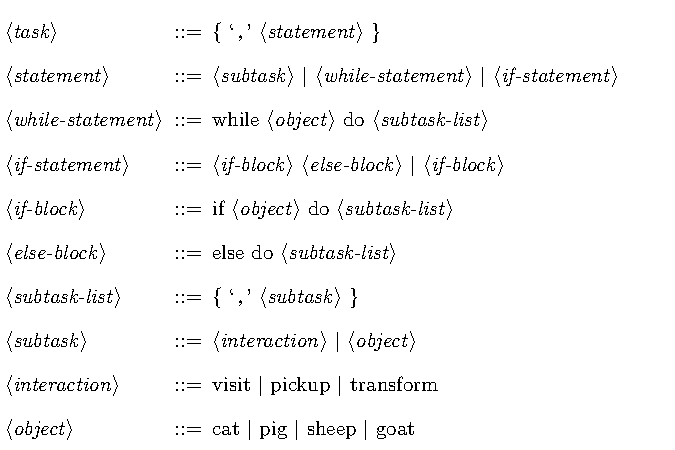
\includegraphics[width=\columnwidth]{grammar}}
\caption{Grammar defining valid instructions}
\label{grammer}
\vskip -0.2in
\end{figure}

\subsection{Environment}
In keeping with \cite{oh2017zero}, our environment consists of a gridworld in which
objects (cat, pig, sheep, goat), are randomly placed. In order to perform a
subtask, the agent must navigate to the object, and perform the appropriate
interaction (visit, pickup, or transform), which each affect the environment in
a different way.


\section{Approach}
\label{approach}
Our goal in this research was not only to develop an architecture capable of
mastering tasks corresponding to complex logical instructions but to generalize
to longer tasks than those on which the agent was trained.
In section \ref{experiments}, we present evidence that conventional architectures
fail to master even the tasks in their training set once those tasks exceed a
certain complexity.
However, simpler architectures than ours do demonstrate strong training
performance.  What sets our architecture apart is
its ability to generalize to longer instructions. Our architecture incorporates three
key insights:

\begin{enumerate}
  \item \textbf{Internal memory pointer:} Borrowing from \cite{oh2017zero}, our architecture incorporates an
    internal memory pointer that learns to track the agent's progress through
    the larger instruction.
  \item \textbf{Instruction Scanning:} When moving the internal memory pointer, the agent
    chooses the next line by ``scanning'' a learned representation of the  instruction and
    jumping to the next occurrence of some information in the learned
    representation, instead of basing the choice of movement on
    the length or direction of movement.
  \item \textbf{Instruction Rolling:} Our agent shifts or ``rolls'' the learned representation of the instruction
    specification so that the agent always chooses movements of the internal memory pointer
    relative to the current active line.
\end{enumerate}

\subsection{Internal memory pointer}
\label{internal-memory-pointer}
As in \cite{oh2017zero}, given a $K$-length instruction and hidden size $H$, the architecture generates a learned instruction memory
$\mathbf{M} \in \mathbb{R}^{K \times H}$ that encodes each instruction $\mathbf{I}$ 
using ``Bag-of-words'' style
encodings applied to each line. Each line is
a list of words $\mathbf{l}_k = \left(w^k_1,\dots,w^k_{|\mathbf{l}_k|}\right)$ and each instruction is
a list of lines $\mathbf{I} = \left(\mathbf{l}_1,\dots,\mathbf{l}_{K}\right)$. Note that a
line may either correspond to a subtask or to a control-flow statement.
In order to generate the instruction memory, each word is embedded and the
embeddings are summed:
\begin{equation}
  \mathbf{M}_k = \sum_{i=1}^{|\mathbf{l}_k|} \phi\left(w^k_i\right)
\end{equation}

In \cite{oh2017zero}, the
upper-level agent chooses 
subtask parameters as a function of a weighted sum of these
embeddings and learns a convolution operator 
that smoothly shifts the attention of these weights left or right by at most one step.

We modify this approach to the internal memory pointer by using hard instead of
soft attention---that is, instead of maintaining a set of weights over all
lines in the instruction, we maintain a single integer pointer $0 \le p_t < K$ 
whose movements are sampled from a learned distribution. We found that this was beneficial, since a smooth shift might
cause the pointer to split along different paths of a conditional statement.

Moreover, because the next line in the instruction may not immediately follow or
precede the current line, we found that it was beneficial to allow the agent to
move the pointer greater distances than a single line. We therefore augment the
possible action space for the internal pointer to include movements to all other
lines in the instruction.

\begin{figure*}[ht]
\centering
  \begin{subfigure}{.3\textwidth}
    \centering
\begin{tikzpicture}[x=0.5mm,y=0.5mm,
    bit/.style={
% The shape:
rectangle,
% The size:
minimum height=.1mm,
minimum width=.1mm,
fill=black
},
    bin/.style={
% The shape:
rectangle,
% The size:
minimum height=8mm,
minimum width=3.5mm,
},
    matrix/.style={
% The shape:
rectangle,
% The size:
minimum height=8mm,
minimum width=28mm,
% The border:
thin, draw,
},
    vector/.style={
% The shape:
rectangle,
% The size:
minimum height=1mm,
minimum width=28mm,
% The border:
thin, draw,
},
      decoration = {snake,   % <-- added
                    pre length=1pt,post length=1pt,% <-- for better looking of arrow,
                    },
                    main matrix/.style = {circle,draw,fill=#1,},
]
  \fill[black!10] (-24,67) rectangle (-20,77);
  \fill[black!30] (-20,67) rectangle (-16,77);
  \fill[black!60] (-16,67) rectangle (-12,77);
  \fill[black!80] (-12,67) rectangle (-8,77);
  \fill[black!30] (-8,67) rectangle (-4,77);
  \fill[black!20] (-4,67) rectangle (0,77);
  \fill[black!40] (0,67) rectangle (4,77);
  \fill[black!15] (4,67) rectangle (8,77);
  \fill[black!10] (12,67) rectangle (16,77);
  \fill[black!30] (16,67) rectangle (20,77);
  \fill[black!70] (20,67) rectangle (24,77);
  \fill[black!40] (24,67) rectangle (28,77);

  \node[bin,opacity=.3,fill=cyan]  at (-24.7, 24) {};
  \node[bin,opacity=.3,fill=green]   at (-17.7, 24) {};
  \node[bin,opacity=.3,fill=yellow]    at (-10.7, 24) {};
  \node[bin,opacity=.3,fill=orange] at (-3.7, 24)  {};
  \node[bin,opacity=.3,fill=red]   at (3.3, 24)   {};
  \node[bin,opacity=.3,fill=purple]    at (10.3, 24)  {};
  \node[bin,opacity=.3,fill=violet]  at (17.3, 24)  {};
  \node[bin,opacity=.3,fill=blue] at (24.3, 24)  {};

  \node[bin,opacity=.3,fill=yellow]    at (-24.7,48) {};
  \node[bin,opacity=.3,fill=orange] at (-17.7,48) {};
  \node[bin,opacity=.3,fill=red]   at (-10.7,48) {};
  \node[bin,opacity=.3,fill=purple]    at (-3.7,48)  {};
  \node[bin,opacity=.3,fill=violet]  at (3.3,48)   {};
  \node[bin,opacity=.3,fill=blue] at (10.3,48)  {};
  \node[bin,opacity=.3,fill=cyan]  at (17.3,48)  {};
  \node[bin,opacity=.3,fill=green]   at (24.3,48)  {};

  %\draw[step=2mm] (-28.1,-4.1) grid (28.1,8.1);
  \node[matrix]                                 (I) at (0, 0)          {Instruction $\mathbf{I}$};
  %\node                                 () at (0, -10)         {Instruction $\mathbf{I}$};
  \node[matrix]                         (M) at (0, 24)         {$\mathbf{M}$};
  \node[matrix]                         (rolled) at (0, 48)    {$\mathbf{M}$};
  \node[vector]                         (B) at (0, 72)         {$\mathbf{B}$};
  \node[]                               (samples) at (0, 86) {};
  \draw[step=2mm] (-28.1,84) grid (28.1,88);

  \fill[black] (-8,84) rectangle (-12,88);
  \fill[black] (0,84) rectangle (4,88);
  \fill[black] (20,84) rectangle (24,88);

  \node[]                               (samples) at (0, 86) {};
  \draw[step=2mm] (-28.1,96) grid (28.1,100);
  \fill[black] (-8,96) rectangle (-12,100);
  \node[]                               (samples1) at (0, 86) {};
  \node[]                               (sample) at (0, 98) {};
  \node[]                               () at (-10, 104) {$d_t$};
  \draw[->] (-28,104) -> node[above] {\tiny choose first} (-14,104);


  \draw[->] (-28,58) -> (28,58);
  \draw[->] (28,60) -> (-28,60);

  \draw[->] (I)      -> node[right] {\tiny embed}             (M);
  \draw[->] (M)      -> node[right] {\tiny roll}              (rolled);
  \draw[->] (rolled) -> node[right,yshift=1mm] {\tiny Bidirectional GRU} (B);
  \draw[->] (B)      -> node[right] {\tiny sample}            (samples);
  %\draw[->] (samples1)      -> node[right] {\tiny sample}            (sample);
\end{tikzpicture}
\caption{\textbf{Generation of transition distributions:} Architecture for
  mapping instruction $\mathbf{I}$ to pointer transition values $d_t$. Note that Note that $\mathbf{P}$ contains $\ell$ such distributions and
$\tilde{\mathbf{u}}_t$ chooses among them.}
  \label{schematic1}
  \end{subfigure}
\hfill
  \begin{subfigure}{.3\textwidth}
    \centering
\begin{tikzpicture}[x=2mm,y=2mm,
    bin/.style={
% The shape:
rectangle,
% The size:
minimum height=8mm,
% The border:
thin, draw,
},
    weight/.style={
% The shape:
rectangle,
% The size:
minimum height=1mm,
% The border:
thin, draw,
},
    weights/.style={
% The shape:
rectangle,
% The size:
minimum height=1mm,
minimum width=24mm,
% The border:
thin, draw,
},
    memory/.style={
% The shape:
rectangle,
% The size:
minimum height=8mm,
minimum width=24mm,
% The border:
thin, draw,
},
      decoration = {snake,   % <-- added
                    pre length=1pt,post length=1pt,% <-- for better looking of arrow,
                    },
                    main node/.style = {circle,draw,fill=#1,},
]
  \node[memory,label={[xshift=-19.0mm]right:Memory $\mathbf{M}$}]
    (M) at (-3, 2) {};
  \node[memory]                         (P) at (5, 22) {$\mathbf{P}$};
  \node at (-7, -1) {$p_t$};
  \node[bin]                            (Mp) at (-7, 2) {};
  \node[minimum size=1cm, draw,circle]  (x) at (6, 2) {$\mathbf{x}_t$};
  \node[draw,circle,minimum size=1cm]   (GRU) at (0, 10) {GRU};
  \fill [black!5]                      (-1,16) rectangle (0.5,18);
  \fill [black!10]                      (0.5,16) rectangle (2,18);
  \fill [black!20]                      (2,16) rectangle (3.5,18);
  \fill [black!10]                      (3.5,16) rectangle (5,18);
  \fill [black!5]                      (5,16) rectangle (6.5,18);
  \draw [decorate,decoration={brace}]
  (-1,18.5) -- (11,18.5) node[midway,yshift=2mm]{\tiny softmax};
  \node[weights]                        (u) at (5, 17) {$\mathbf{u}_t$};
  \node                                 (p1) at (5, 30) {$d_{t}$};
  \node                                 (g) at (-5, 17) {$\mathbf{g}_t$};
  %\node                                 (cat) at (15, 30)
  %{$\Cat\left(\mathbf{P}\tilde{\mathbf{u}}_t\right)$};

  \draw [decorate,decoration={brace}]
  (-1,24.5) -- (11,24.5) node[midway,yshift=2mm]{};
  \node   (weighted-sum) at (5, 25.5) {\tiny weighted-sum};

  \draw [->] (Mp)          to [out=90,in=225] (GRU);
  \draw [->] (x)          to [out=90,in=315] (GRU);
  \draw [->] (GRU) to [out=135,in=270] node[left] {\tiny sample} (g);
  \draw [->] (GRU) to [out=45,in=270] (u);
  \draw [->] (GRU) edge[loop right] node {$\mathbf{h}_t$} (h);
  %\draw[->] (weighted-sum) -> (cat);
  \draw[->] (weighted-sum) -> node[right] {\tiny sample} (p1);

\end{tikzpicture}
\caption{\textbf{Schematic for our architecture:} Diagram of architecture that maps the
observation $\mathbf{x}_t$ and current memory pointer $p_t$ to the pointer delta
$d_t$. Note that $p_{t+1} = p_t + d_t$.}
\end{subfigure}
\hfill
\begin{subfigure}{.3\textwidth}
  \centering
\begin{tikzpicture}[x=2mm,y=2mm,
    bin/.style={
% The shape:
rectangle,
% The size:
minimum height=8mm,
% The border:
thin, draw,
},
    memory/.style={
% The shape:
rectangle,
% The size:
minimum height=8mm,
minimum width=24mm,
% The border:
thin, draw,
},
      decoration = {snake,   % <-- added
                    pre length=1pt,post length=1pt,% <-- for better looking of arrow,
                    },
                    main node/.style = {circle,draw,fill=#1,},
]
  \node[memory] (I) at (-5, -10) {$\mathbf{I}$};
  \node[memory] (M) at (-5, -4) {$\mathbf{M}$};
  \node[bin] (H) at (-5, 2) {$\mathbf{H}'$};
  \node[minimum size=1cm, draw,circle]  (x) at (6, 2) {$\mathbf{x}_t$};
  \node                                 (g) at (0, 17) {$\mathbf{g}_t$};
  \node[draw,circle,minimum size=1cm]   (GRU) at (0, 10) {GRU};
  \draw [->] (I)  -> node[right] {\tiny embed} (M);
  \draw [->] (M)  -> node[right] {\tiny Bidirectional GRU} (H);
  \draw [->] (H)  to [out=90,in=225] (GRU);
  \draw [->] (x)   to [out=90,in=315] (GRU);
  \draw [->] (GRU) -> node[right] {\tiny sample} (g);
  \draw [->] (GRU) edge[loop right] node {$\mathbf{h}_t$} (h);

\end{tikzpicture}
\caption{Diagram of \textbf{No pointer} baseline architecture.}
\label{no-pointer}
\end{subfigure}
\end{figure*}

\subsection{Instruction Scanning}\label{scanning}
Each episode, our architecture generates a graph representation of the
instruction that allows the internal memory to navigate the instruction over the
course of the episode.  From every line in the instruction, we produce
$\ell$ outgoing edges which each correspond to a learned distribution over other lines
in the instruction. To produce each distribution, we feed the embedded representation
of the instruction $\mathbf{M}$ through a bidirectional GRU to produce a
representation $\mathbf{H} \in \mathbb{R}^{2K \times H}$ of the instruction
that incorporates local context information. The outputs of the GRU in both
directions are projected to a vector $\mathbf{B} \in (0, 1)^{2K\times \ell
 }$ using a sigmoidal
perceptron. Finally the equation for the distribution over next lines is
\begin{equation}
  \label{P}
  \mathbf{P}_{ij} = \mathbf{B}_{ij}\prod_{k \in (1, -1, 2, -2, \dots)}\left(1 -
  \mathbf{B}_{kj}\right)
\end{equation}
where $\mathbf{P} \in \mathbb{R}^{2K\times\ell }$. Intuitively, $\mathbf{P}$ is the distribution produced by
sampling a Bernoulli distribution parameterized by $\mathbf{B}_k$ at each index
$k$, concentrically moving away from the first index, and stopping at the first success.

As in \cite{oh2017zero}, movements of the internal memory pointer are a learned
function of the history of selections in memory, of actions and of observations.
Concretely, we generate a hidden state by feeding all of these values each time
step through a Gated Recurrent Network \cite{ChoMGBSB14}:
\begin{equation}
  \mathbf{h}_t = \GRU\left(f_\theta\left(\mathbf{x}_t\right),
    \mathbf{M}_{p_{t-1}}, \mathbf{g}_{t-1},
  \mathbf{h}_{t-1}\right)
\end{equation}
where $f_\theta$ is a convolutional neural network. Whereas \cite{oh2017zero}
projects $\mathbf{h}_{t}$ to the one-step convolution operator described in
section \ref{internal-memory-pointer}, we project $\mathbf{h}_t$ to $\mathbf{u}_t\in \mathbb{R}^\ell$, a weight vector
used to choose among paths previously encoded from the instruction. Thus the final
distribution over next lines is
$\Cat(\mathbf{P}_{p_t}\tilde{\mathbf{u}}_t)$, where $\tilde{\mathbf{u}}_t =
\softmax\left(\mathbf{u}_t\right)$.

\subsection{Instruction Rolling}
This feature takes advantage of the fact that the rules of control flow are
invariant to the position of the current line in the instruction. ``Rolling'' here
refers to a modular operation by which all elements in a tensor are shifted in
one direction such that elements shifted beyond the last position are
re-introduced at the first position. For example, rolling the tensor 
$\begin{bmatrix} 1 & 2 & 3 & 4 & 5 \end{bmatrix}$ by $-2$ generates the tensor
$\begin{bmatrix} 3 & 4 & 5 & 1 & 2 \end{bmatrix}$. 

The relevance to our architecture is that the encoded instruction $\mathbf{M}$ is rolled to the current memory index
$p_t$ before feeding it to the bidirectional GRU. In other words, the forward GRU takes lines in the
order $(p_t, p_t + 1, \dots, K, 1, \dots, p_t - 1)$, running from the current
line, wrapping around the last line of the instruction, and returning to the line
before the current line. Thus the operations described in section \ref{scanning} are all performed
relative to the current active line in memory. That is, $\mathbf{B}_{i}$ in
equation \ref{P} refers to the row of $\mathbf{B}$ corresponding to the $(p_t +
i)^{\text{th}}$ index of $\mathbf{M}$ .

\algo{Subtask update}{
    \STATE $\mathbf{M}^{p_t} \gets \roll\left(\mathbf{M}, -p_t\right)$
    %\COMMENT{roll function rotates $\mathbf{M}$ around first
    %axis. $\mathbf{M}_t \in \mathbb{R}^h$}
    \STATE ${\mathbf{H}_t} \gets \BIGRU\left(\mathbf{M}^{p_t}\right)$
    %\COMMENT{{$\mathbf{H}_t \in \mathbb{R}^{2n \times w \times h}$}}
    \STATE ${\mathbf{P}_t \gets \scan\left(\mathbf{H}_t\right)}$
    %\COMMENT{$\mathbf{P}_t$ comprises $\ell$ $2K$-dimensional probability
    %distributions}
}{}{}
\begin{algorithm}[b]
  \caption{Scan Function}
  \label{scan}
  \begin{algorithmic}[1]
   \STATE {\bfseries Inputs:} 
$\mathbf{H} \in \mathbb{R}^{2K \times H}$ 
%\STATE $\mathbf{B} \gets \sigma\left(\Call{MLP}{\mathbf{H}}\right)$
%\COMMENT{$\mathbf{B}\in \mathbb{R}^{a \times w}$}
\STATE $\mathbf{B}_{-1} \gets 1$  
\STATE initialize $\mathbf{P} \in \mathbb{R}^{2K \times \ell}$
\FOR{$i$ in $0, \dots, 2K$}
\STATE $\mathbf{P}_i \gets \mathbf{B}_i\prod_{j=1}^{i-1}\left(1 - \mathbf{B}_j\right)$
%\COMMENT{This expression ensures the columns of $\mathbf{W} \in
%\mathbb{R}^{2n}$.}
\ENDFOR
\STATE return $\mathbf{P}$
  \end{algorithmic}
\end{algorithm}

\begin{figure*}[]
  \centering
  \begin{subfigure}{.33\textwidth}
    \centering
    \centerline{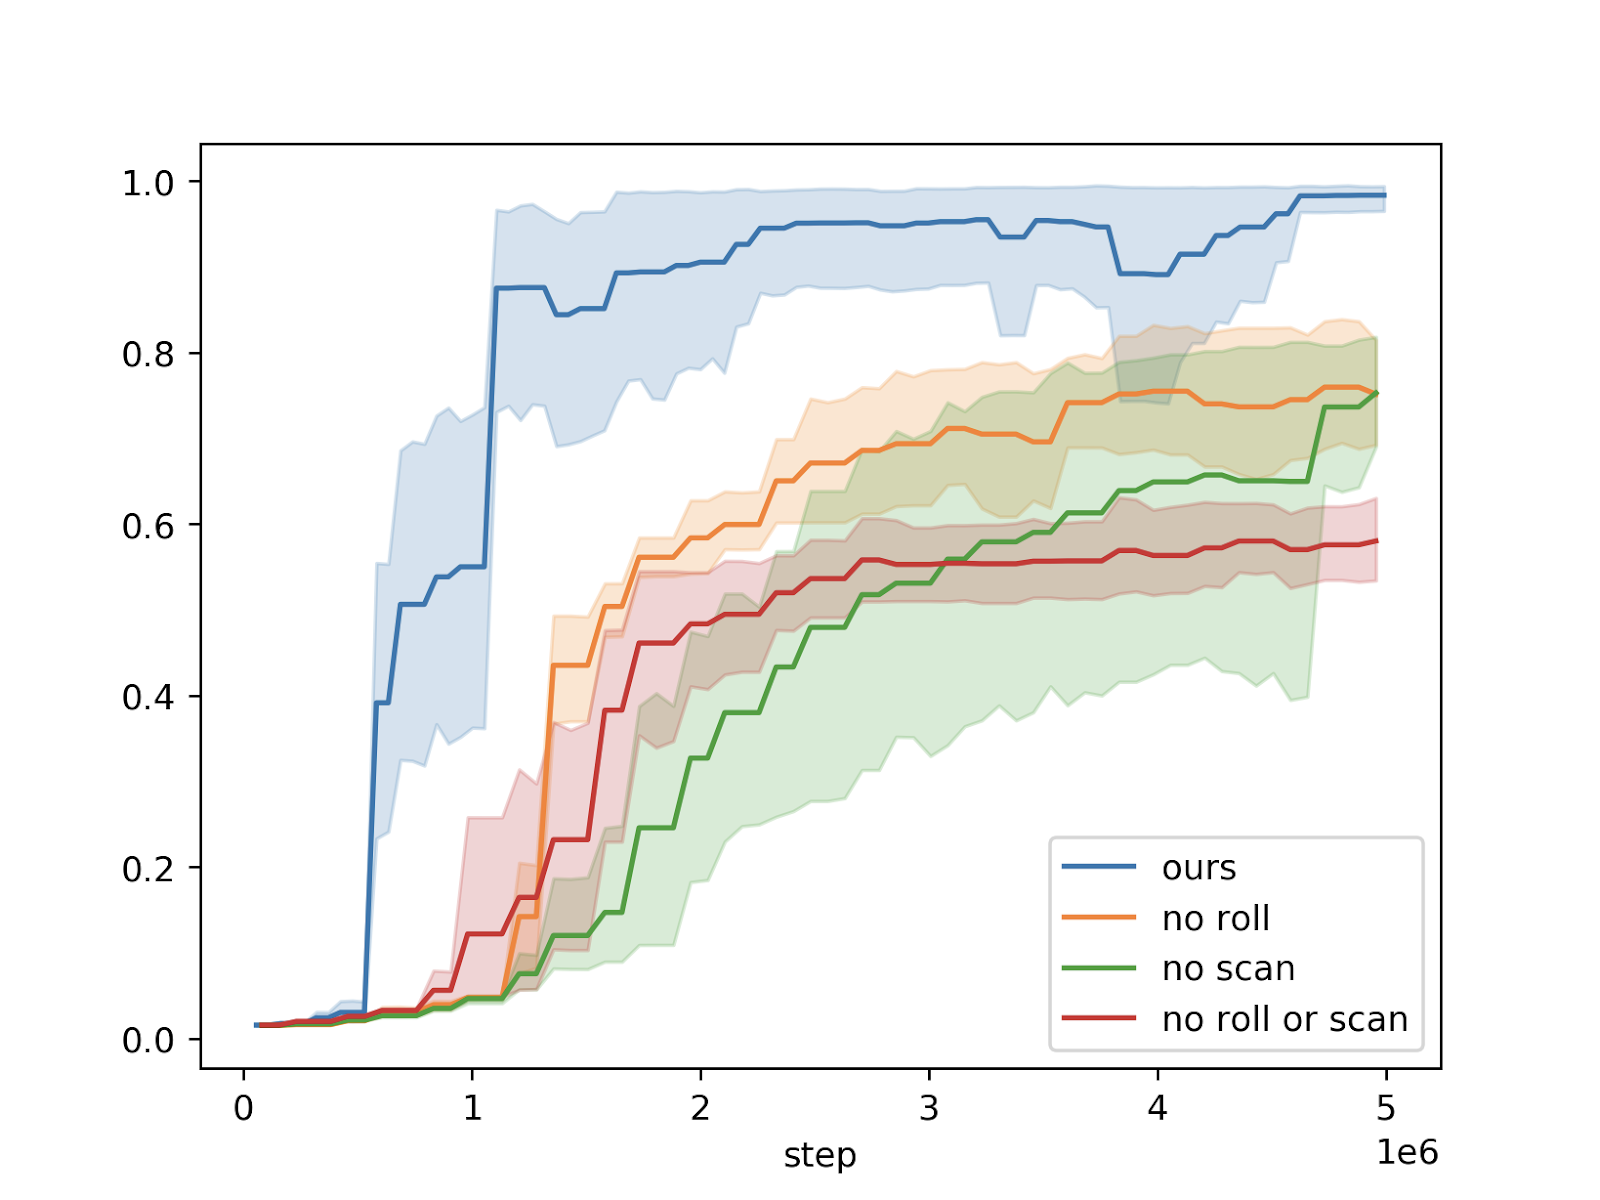
\includegraphics[trim=100 0 100 100, clip, width=\columnwidth]{figures/eval20}}
    \caption{Evaluation on instructions of length 20}
  \end{subfigure}%
  \begin{subfigure}{.33\textwidth}
    \centering
    \centerline{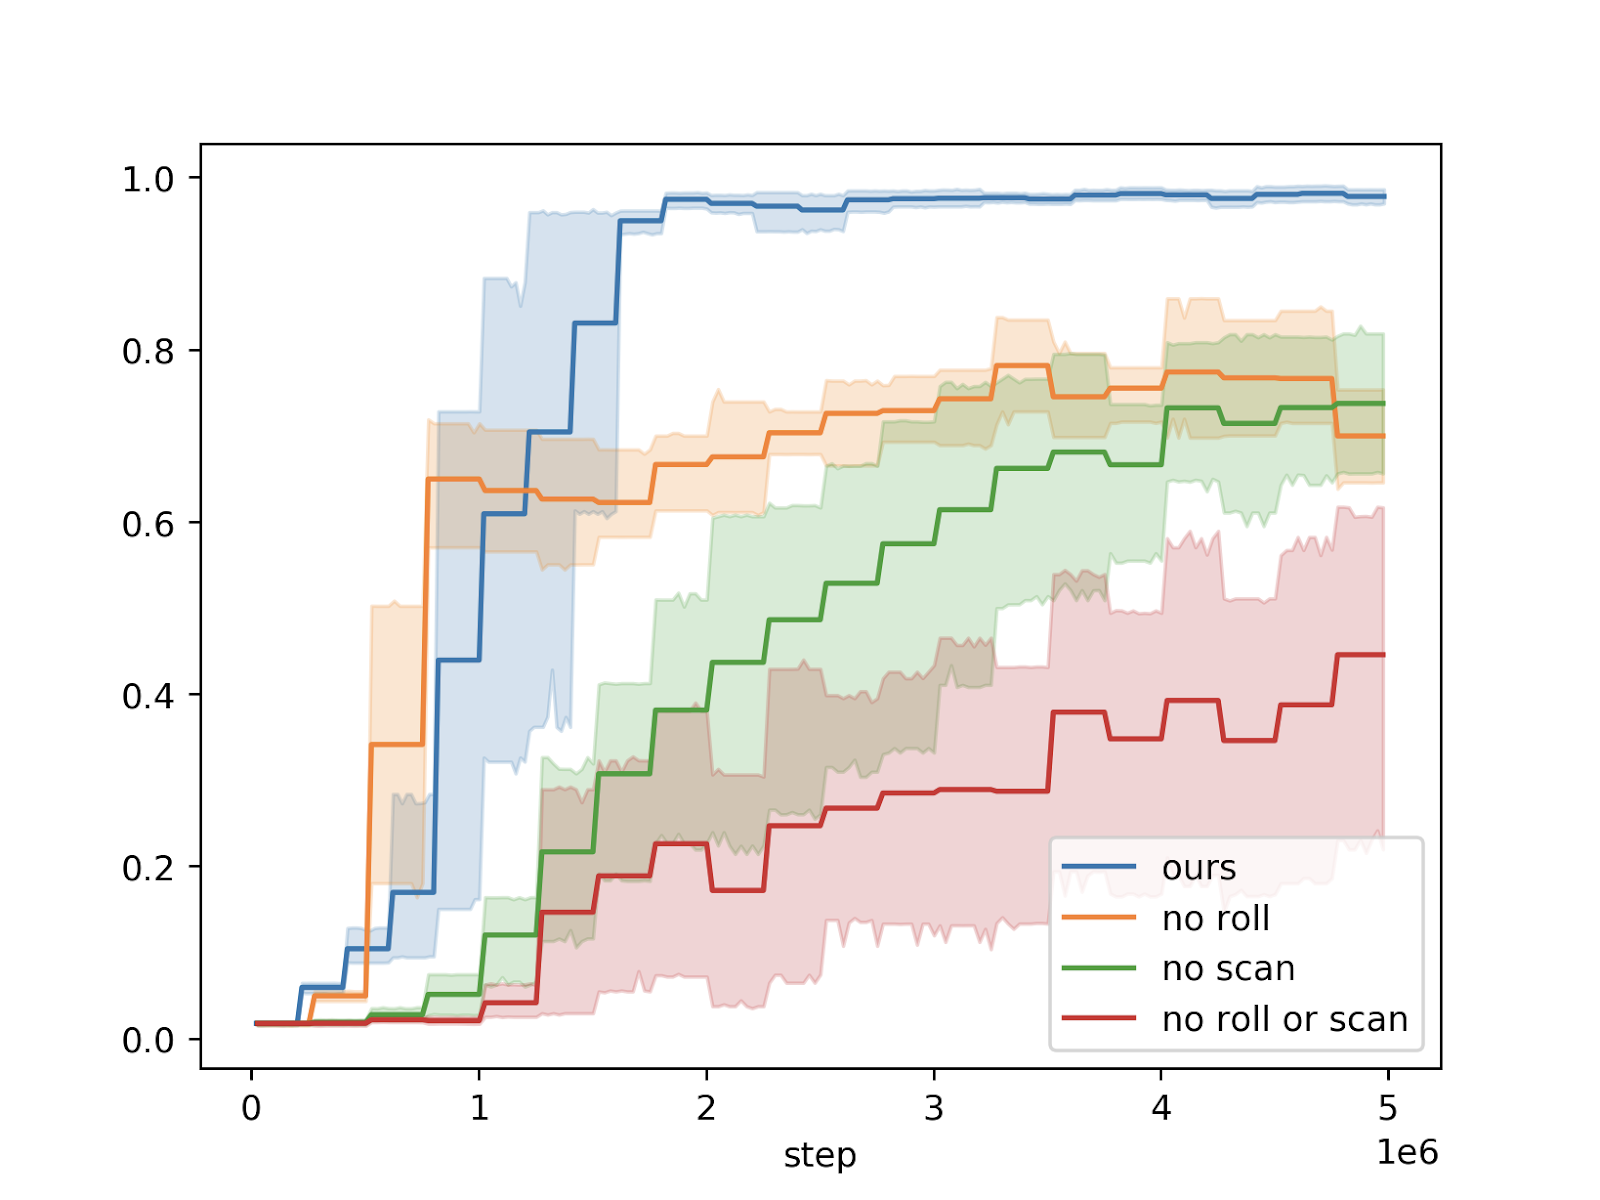
\includegraphics[trim=100 0 100 100, clip, width=\columnwidth]{figures/eval30}}
    \caption{Evaluation on instructions of length 30}
  \end{subfigure}%
  \begin{subfigure}{.33\textwidth}
    \centering
    \centerline{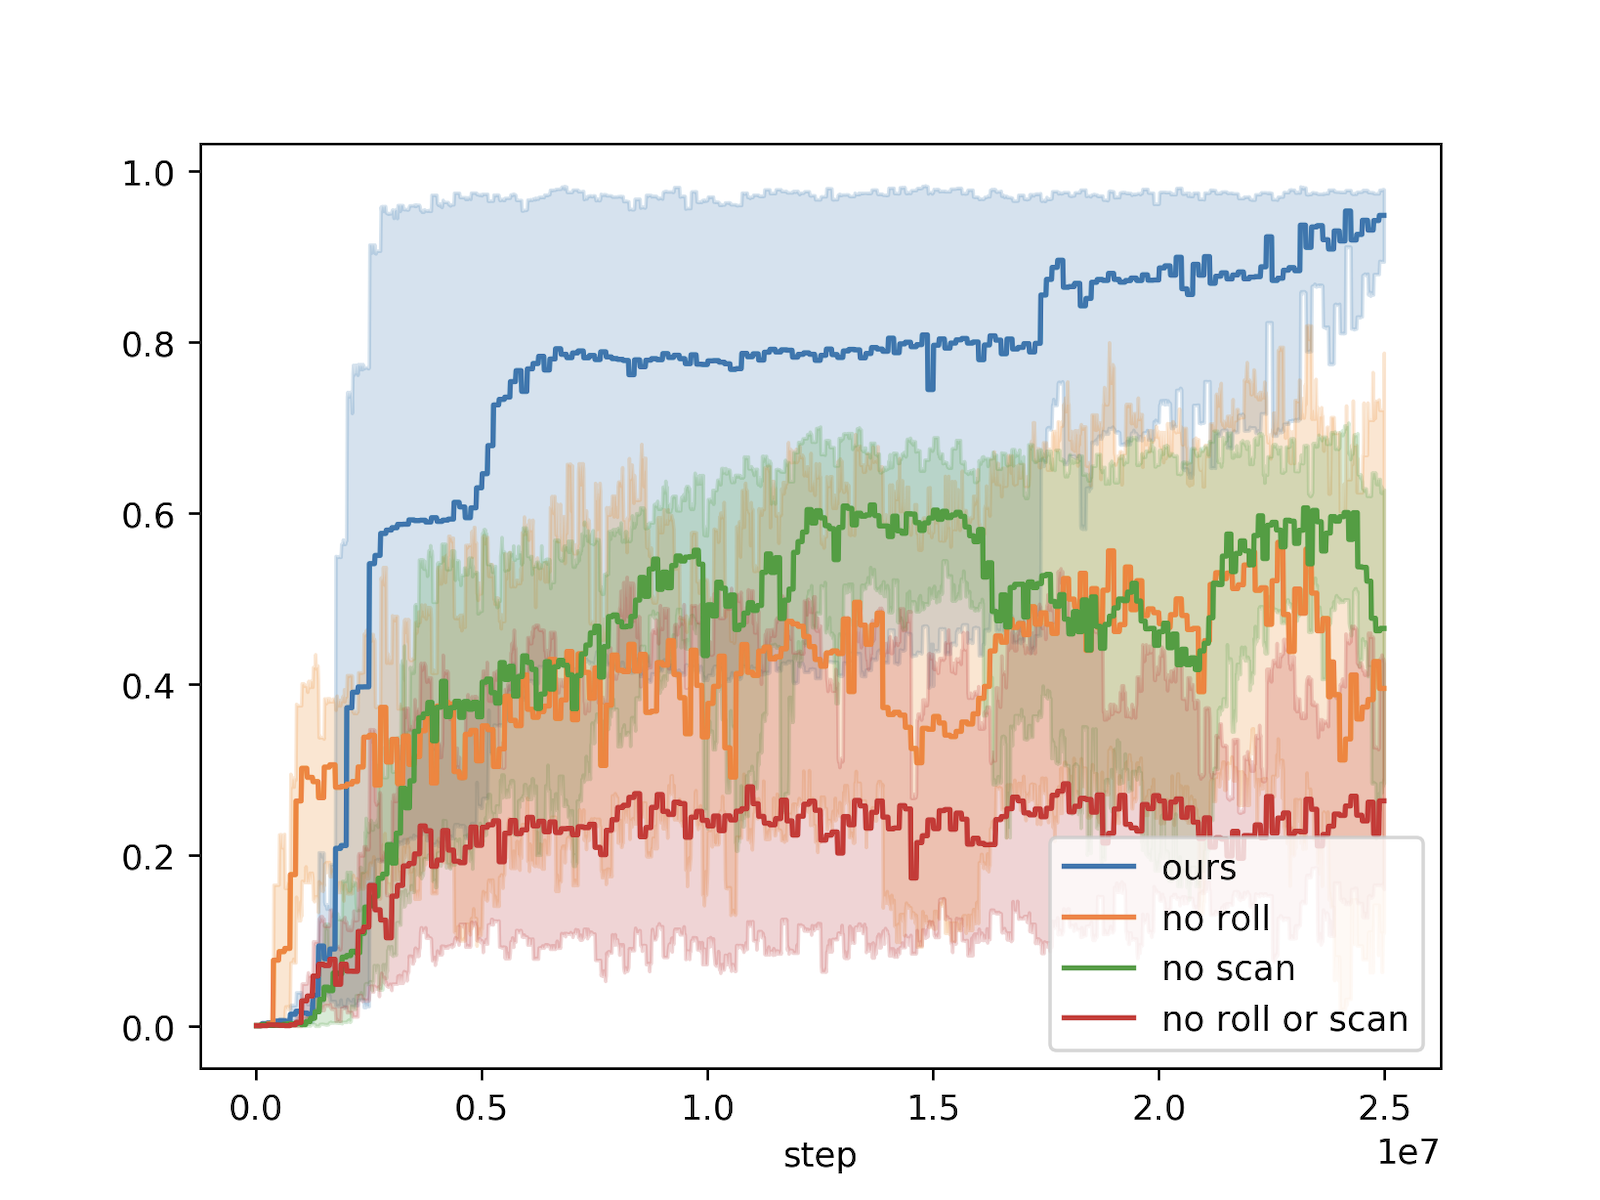
\includegraphics[trim=100 0 100 100, clip, width=\columnwidth]{figures/eval40}}
    \caption{Evaluation on instructions of length 40}
  \end{subfigure}%
  \caption{Each graph demonstrates the capability of the agent to generalize to
  longer instruction lengths on the minimal environment. Details are provided in
section \ref{results}.}
  \label{minimal}
\end{figure*}

\section{Experiments}
\label{experiments}
In order to validate the effectiveness of our algorithm, we ran two sets of
experiments in different environments. The first environment is minimal,
intended only to test
the agent's capability to move the internal memory pointer through an instruction
involving complex control flow. The second involves temporally-extended subtasks
of the kind discussed earlier and non-trivial logical conditions.

\subsection{Baselines}
In our experiments, we ablate the main features of our algorithm in order to
test their effectiveness. We present five baselines:
\begin{itemize}
  \item \textbf{No scan:} This baseline removes the instruction scanning feature by
    taking the last output of $\BIGRU(\mathbf{M}^{p_t})$ and projecting it to
    a distribution over possible forward and backward pointer movements.
    Movements that go beyond the beggining or end of the instruction are clipped.
  \item \textbf{No roll:} This baseline does not roll $\mathbf{M}$ before feeding
    it to the bidirectional GRU.
  \item \textbf{No roll or scan:} This baseline combines both ablations.
  \item \textbf{No pointer:} This baseline removes the internal memory pointer.
    Instead, it feeds a representation $\mathbf{H}'$ of the instruction
    $\mathbf{I}$ along with the observation $\mathbf{x}_t$ to a GRU controller
    which directly outputs a distribution over actions $\pi_\theta(\cdot)$ and a
    value $V_t$. We generate $\mathbf{H}'$ by feeding the embedded instruction
    $\mathbf{M}$ through a bidirectional GRU and concatenating the last outputs
    in both directions. See figure \ref{no-pointer}.
  \item \textbf{Oh et. al.} This baseline reproduces the algorithm described in
    \cite{oh2017zero}.
\end{itemize}
 Psuedocode for all the baselines is also included in Appendix A.

\subsection{Minimal Environment}
In the minimal setting, subtasks are not
temporally extended -- as soon as the agent outputs the correct subtask
parameter, the subtask is complete and the external program counter advances.
Moreover, conditions are evaluated according to a simple ``condition bit'' which
is randomly 1 or 0, with 50\% probability. If the condition bit is 1,
\texttt{if}-conditions and \texttt{while}-conditions pass, otherwise they fail.

\subsection{Complex Environment}
In this setting, the agent dictates subtask parameters to a pretrained
lower-level agent who executes them. Thus subtasks may take several time-steps to
complete. Moreover, conditions are parameterized by \textit{objects} and they
are evaluated according to whether the object exists. For example, the statement
\texttt{If cat} evaluates to true, if there is a cat somewhere in the
environment, and false otherwise.
\begin{figure}[t]
\vskip 0.2in
\centerline{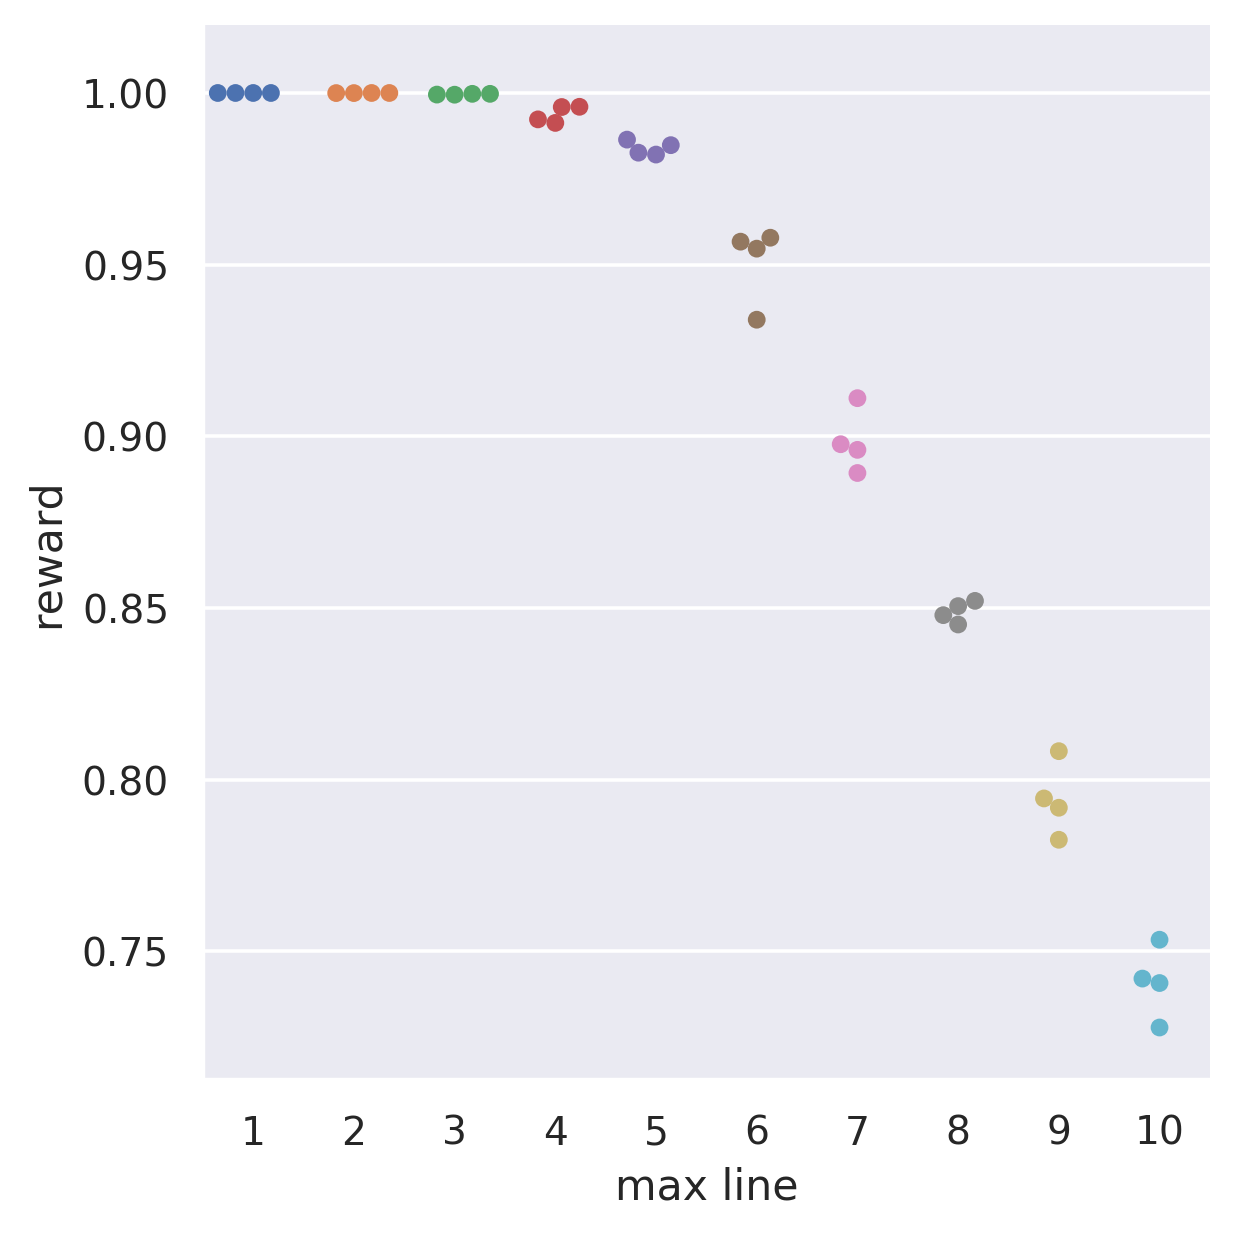
\includegraphics[width=\columnwidth]{gru_rewards}}
\caption{This graph compares the performance of our architecture with the
baseline architectures on tasks twice as long as those trained (20 lines).
Details are provided in section \ref{results}.}
\label{complex}
\vskip -0.2in
\end{figure}

\begin{figure}[t]
\vskip 0.2in
\centerline{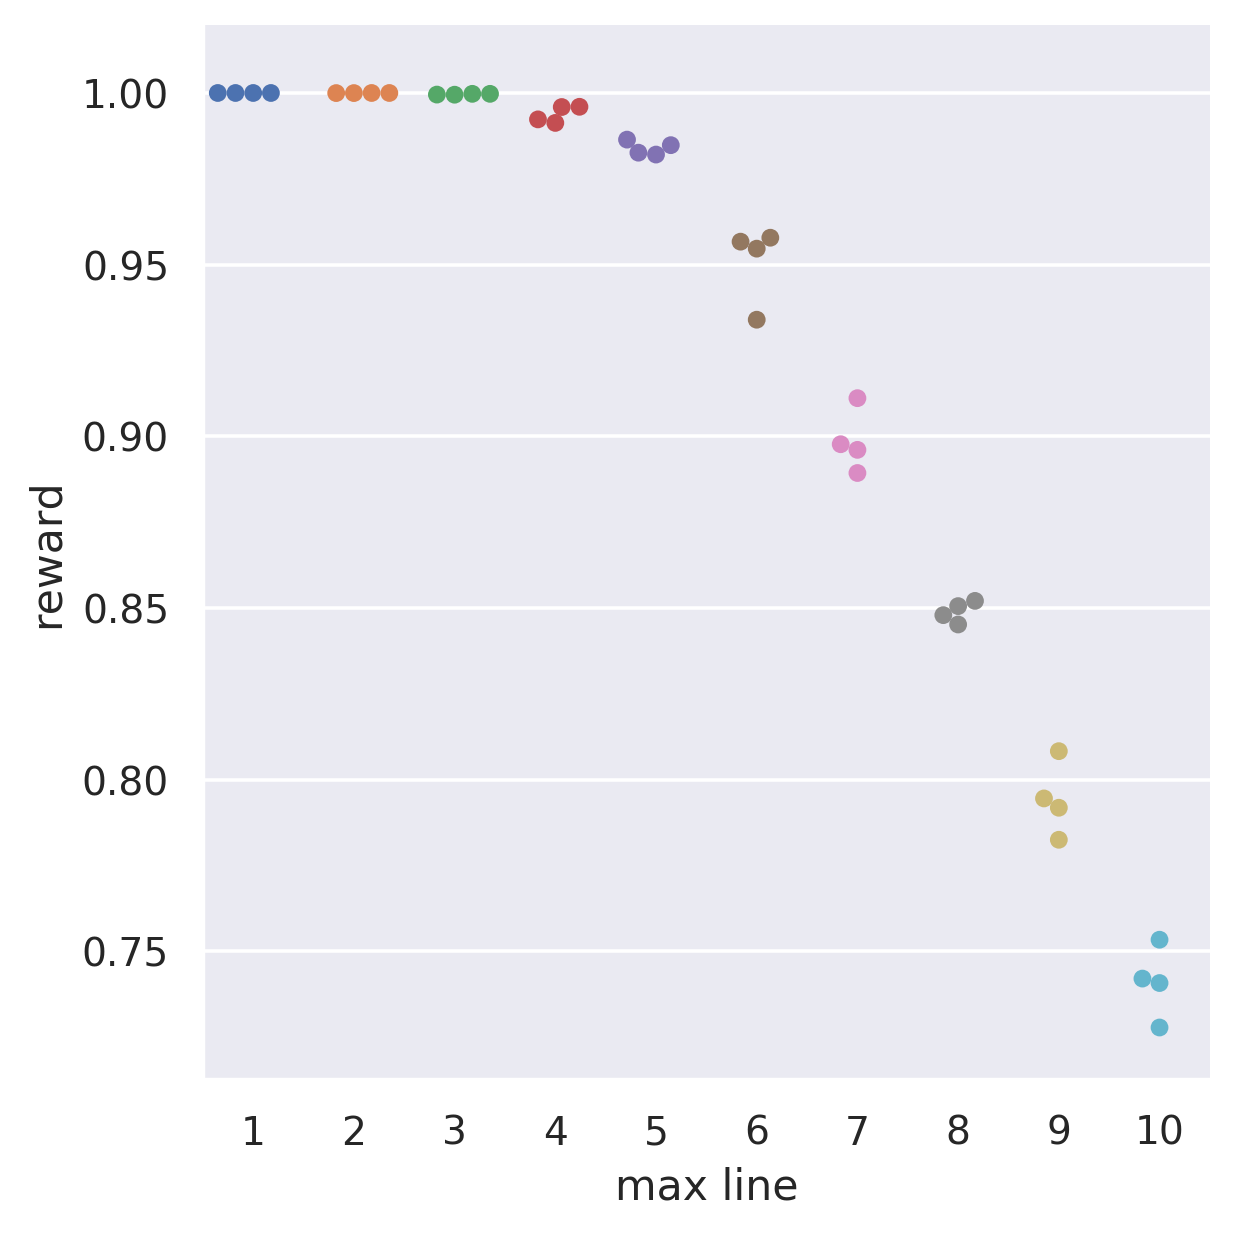
\includegraphics[width=\columnwidth]{gru_rewards}}
\caption{This graph depicts the degradation in \textit{training} performance of the minimal
\textbf{No Pointer} baseline architecture on minimal environment. The $x$-axis
depicts the maximum lines per instruction for each experiment (each episode the
number of lines is drawn unifomly at random from between one and this number).
The $y$-axis depicts the average cumulative training reward averaged across 150
parallel processes after 13 million gradient updates. This number was chosen by
visually }
\label{gru-rewards}
\vskip -0.2in
\end{figure}

\subsection{Results}
\label{results}
Figures \ref{minimal} and \ref{complex} compare the performance of our
architecture with several baselines. 
Each graph plots the rewards that these architectures achieved on \textit{longer
length} instructions.
 Note that all graphs depict the performance of agents trained on instructions with lengths drawn uniformly between 1 and 10. Thus
the graphs measure the generalization capability of each architecture. Each
line is the average reward achieved by 150 parallel processes over the course of
200 steps of evaluation. The error bars represent five separate distinct random
seeds ($150 \times 5$ total processes).

\subsection{Analysis}
To do

\section{Conclusion}
This work studies a special but important subset of multi-task reinforcement
learning problems, namely instructions with complex control-flow. We consider
problems of this nature an important stepping stone toward natural language
instructions and toward agents capable of arbitrarily complex logic. We hope
that future work will explore instructions that involve greater complexity,
including conditionals with more complex predicates, higher-dimensional
observations, and noisy natural-language inputs.

\section{To do}
\begin{itemize}
  \item Write results section
  \item Failure analysis
  \item Improve figure \ref{schematic1}
  \item fill out appendix
  \item Add more related works
  \item Add diagram of edge length performance.
  \item Replace figure \ref{gru-rewards} once runs are complete
  \item Add diagram of performance on 6x6 environment once runs are complete.
  \item If time permits, add other baselines to single-step environment.
\end{itemize}

%\section{Electronic Submission}
%\label{submission}

%Submission to ICML 2019 will be entirely electronic, via a web site
%(not email). Information about the submission process and \LaTeX\ templates
%are available on the conference web site at:
%\begin{center}
%\textbf{\texttt{http://icml.cc/}}
%\end{center}

%The guidelines below will be enforced for initial submissions and
%camera-ready copies. Here is a brief summary:
%\begin{itemize}
%\item Submissions must be in PDF\@.
%\item The maximum paper length is \textbf{8 pages excluding references and
    %acknowledgements, and 12 pages including references and acknowledgements}
    %(pages 9 through 12 must contain only references and acknowledgements).
%\item \textbf{Do not include author information or acknowledgements} in your
    %initial submission.
%\item Your paper should be in \textbf{10 point Times font}.
%\item Make sure your PDF file only uses Type-1 fonts.
%\item Place figure captions \emph{under} the figure (and omit titles from inside
    %the graphic file itself). Place table captions \emph{over} the table.
%\item References must include page numbers whenever possible and be as complete
    %as possible. Place multiple citations in chronological order.
%\item Do not alter the style template; in particular, do not compress the paper
    %format by reducing the vertical spaces.
%\item Keep your abstract brief and self-contained, one paragraph and roughly
    %4--6 sentences. Gross violations will require correction at the
    %camera-ready phase. The title should have content words capitalized.
%\end{itemize}

%\subsection{Submitting Papers}

%\textbf{Paper Deadline:} The deadline for paper submission that is
%advertised on the conference website is strict. If your full,
%anonymized, submission does not reach us on time, it will not be
%considered for publication. There is no separate abstract submission.

%\textbf{Anonymous Submission:} ICML uses double-blind review: no identifying
%author information may appear on the title page or in the paper
%itself. Section~\ref{author info} gives further details.

%\textbf{Simultaneous Submission:} ICML will not accept any paper which,
%at the time of submission, is under review for another conference or
%has already been published. This policy also applies to papers that
%overlap substantially in technical content with conference papers
%under review or previously published. ICML submissions must not be
%submitted to other conferences during ICML's review period. Authors
%may submit to ICML substantially different versions of journal papers
%that are currently under review by the journal, but not yet accepted
%at the time of submission. Informal publications, such as technical
%reports or papers in workshop proceedings which do not appear in
%print, do not fall under these restrictions.

%\medskip

%Authors must provide their manuscripts in \textbf{PDF} format.
%Furthermore, please make sure that files contain only embedded Type-1 fonts
%(e.g.,~using the program \texttt{pdffonts} in linux or using
%File/DocumentProperties/Fonts in Acrobat). Other fonts (like Type-3)
%might come from graphics files imported into the document.

%Authors using \textbf{Word} must convert their document to PDF\@. Most
%of the latest versions of Word have the facility to do this
%automatically. Submissions will not be accepted in Word format or any
%format other than PDF\@. Really. We're not joking. Don't send Word.

%Those who use \textbf{\LaTeX} should avoid including Type-3 fonts.
%Those using \texttt{latex} and \texttt{dvips} may need the following
%two commands:

%{\footnotesize
%\begin{verbatim}
%dvips -Ppdf -tletter -G0 -o paper.ps paper.dvi
%ps2pdf paper.ps
%\end{verbatim}}
%It is a zero following the ``-G'', which tells dvips to use
%the config.pdf file. Newer \TeX\ distributions don't always need this
%option.

%Using \texttt{pdflatex} rather than \texttt{latex}, often gives better
%results. This program avoids the Type-3 font problem, and supports more
%advanced features in the \texttt{microtype} package.

%\textbf{Graphics files} should be a reasonable size, and included from
%an appropriate format. Use vector formats (.eps/.pdf) for plots,
%lossless bitmap formats (.png) for raster graphics with sharp lines, and
%jpeg for photo-like images.

%The style file uses the \texttt{hyperref} package to make clickable
%links in documents. If this causes problems for you, add
%\texttt{nohyperref} as one of the options to the \texttt{icml2019}
%usepackage statement.


%\subsection{Submitting Final Camera-Ready Copy}

%The final versions of papers accepted for publication should follow the
%same format and naming convention as initial submissions, except that
%author information (names and affiliations) should be given. See
%Section~\ref{final author} for formatting instructions.

%The footnote, ``Preliminary work. Under review by the International
%Conference on Machine Learning (ICML). Do not distribute.'' must be
%modified to ``\textit{Proceedings of the
%$\mathit{36}^{th}$ International Conference on Machine Learning},
%Long Beach, USA, 2019.
%Copyright 2019 by the author(s).''

%For those using the \textbf{\LaTeX} style file, this change (and others) is
%handled automatically by simply changing
%$\mathtt{\backslash usepackage\{icml2019\}}$ to
%$$\mathtt{\backslash usepackage[accepted]\{icml2019\}}$$
%Authors using \textbf{Word} must edit the
%footnote on the first page of the document themselves.

%Camera-ready copies should have the title of the paper as running head
%on each page except the first one. The running title consists of a
%single line centered above a horizontal rule which is $1$~point thick.
%The running head should be centered, bold and in $9$~point type. The
%rule should be $10$~points above the main text. For those using the
%\textbf{\LaTeX} style file, the original title is automatically set as running
%head using the \texttt{fancyhdr} package which is included in the ICML
%2019 style file package. In case that the original title exceeds the
%size restrictions, a shorter form can be supplied by using

%\verb|\icmltitlerunning{...}|

%just before $\mathtt{\backslash begin\{document\}}$.
%Authors using \textbf{Word} must edit the header of the document themselves.

%\section{Format of the Paper}

%All submissions must follow the specified format.

%\subsection{Length and Dimensions}

%Papers must not exceed eight (8) pages, including all figures, tables,
%and appendices, but excluding references and acknowledgements. When references and acknowledgements are included,
%the paper must not exceed ten (10) pages.
%Acknowledgements should be limited to grants and people who contributed to the paper.
%Any submission that exceeds
%this page limit, or that diverges significantly from the specified format,
%will be rejected without review.

%The text of the paper should be formatted in two columns, with an
%overall width of 6.75~inches, height of 9.0~inches, and 0.25~inches
%between the columns. The left margin should be 0.75~inches and the top
%margin 1.0~inch (2.54~cm). The right and bottom margins will depend on
%whether you print on US letter or A4 paper, but all final versions
%must be produced for US letter size.

%The paper body should be set in 10~point type with a vertical spacing
%of 11~points. Please use Times typeface throughout the text.

%\subsection{Title}

%The paper title should be set in 14~point bold type and centered
%between two horizontal rules that are 1~point thick, with 1.0~inch
%between the top rule and the top edge of the page. Capitalize the
%first letter of content words and put the rest of the title in lower
%case.

%\subsection{Author Information for Submission}
%\label{author info}

%ICML uses double-blind review, so author information must not appear. If
%you are using \LaTeX\/ and the \texttt{icml2019.sty} file, use
%\verb+\icmlauthor{...}+ to specify authors and \verb+\icmlaffiliation{...}+ to specify affiliations. (Read the TeX code used to produce this document for an example usage.) The author information
%will not be printed unless \texttt{accepted} is passed as an argument to the
%style file.
%Submissions that include the author information will not
%be reviewed.

%\subsubsection{Self-Citations}

%If you are citing published papers for which you are an author, refer
%to yourself in the third person. In particular, do not use phrases
%that reveal your identity (e.g., ``in previous work \cite{langley00}, we
%have shown \ldots'').

%Do not anonymize citations in the reference section. The only exception are manuscripts that are
%not yet published (e.g., under submission). If you choose to refer to
%such unpublished manuscripts \cite{anonymous}, anonymized copies have
%to be submitted
%as Supplementary Material via CMT\@. However, keep in mind that an ICML
%paper should be self contained and should contain sufficient detail
%for the reviewers to evaluate the work. In particular, reviewers are
%not required to look at the Supplementary Material when writing their
%review.

%\subsubsection{Camera-Ready Author Information}
%\label{final author}

%If a paper is accepted, a final camera-ready copy must be prepared.
%%
%For camera-ready papers, author information should start 0.3~inches below the
%bottom rule surrounding the title. The authors' names should appear in 10~point
%bold type, in a row, separated by white space, and centered. Author names should
%not be broken across lines. Unbolded superscripted numbers, starting 1, should
%be used to refer to affiliations.

%Affiliations should be numbered in the order of appearance. A single footnote
%block of text should be used to list all the affiliations. (Academic
%affiliations should list Department, University, City, State/Region, Country.
%Similarly for industrial affiliations.)

%Each distinct affiliations should be listed once. If an author has multiple
%affiliations, multiple superscripts should be placed after the name, separated
%by thin spaces. If the authors would like to highlight equal contribution by
%multiple first authors, those authors should have an asterisk placed after their
%name in superscript, and the term ``\textsuperscript{*}Equal contribution"
%should be placed in the footnote block ahead of the list of affiliations. A
%list of corresponding authors and their emails (in the format Full Name
%\textless{}email@domain.com\textgreater{}) can follow the list of affiliations.
%Ideally only one or two names should be listed.

%A sample file with author names is included in the ICML2019 style file
%package. Turn on the \texttt{[accepted]} option to the stylefile to
%see the names rendered. All of the guidelines above are implemented
%by the \LaTeX\ style file.

%\subsection{Abstract}

%The paper abstract should begin in the left column, 0.4~inches below the final
%address. The heading `Abstract' should be centered, bold, and in 11~point type.
%The abstract body should use 10~point type, with a vertical spacing of
%11~points, and should be indented 0.25~inches more than normal on left-hand and
%right-hand margins. Insert 0.4~inches of blank space after the body. Keep your
%abstract brief and self-contained, limiting it to one paragraph and roughly 4--6
%sentences. Gross violations will require correction at the camera-ready phase.

%\subsection{Partitioning the Text}

%You should organize your paper into sections and paragraphs to help
%readers place a structure on the material and understand its
%contributions.

%\subsubsection{Sections and Subsections}

%Section headings should be numbered, flush left, and set in 11~pt bold
%type with the content words capitalized. Leave 0.25~inches of space
%before the heading and 0.15~inches after the heading.

%Similarly, subsection headings should be numbered, flush left, and set
%in 10~pt bold type with the content words capitalized. Leave
%0.2~inches of space before the heading and 0.13~inches afterward.

%Finally, subsubsection headings should be numbered, flush left, and
%set in 10~pt small caps with the content words capitalized. Leave
%0.18~inches of space before the heading and 0.1~inches after the
%heading.

%Please use no more than three levels of headings.

%\subsubsection{Paragraphs and Footnotes}

%Within each section or subsection, you should further partition the
%paper into paragraphs. Do not indent the first line of a given
%paragraph, but insert a blank line between succeeding ones.

%You can use footnotes\footnote{Footnotes
%should be complete sentences.} to provide readers with additional
%information about a topic without interrupting the flow of the paper.
%Indicate footnotes with a number in the text where the point is most
%relevant. Place the footnote in 9~point type at the bottom of the
%column in which it appears. Precede the first footnote in a column
%with a horizontal rule of 0.8~inches.\footnote{Multiple footnotes can
%appear in each column, in the same order as they appear in the text,
%but spread them across columns and pages if possible.}

%\begin{figure}[ht]
%\vskip 0.2in
%\begin{center}
%\centerline{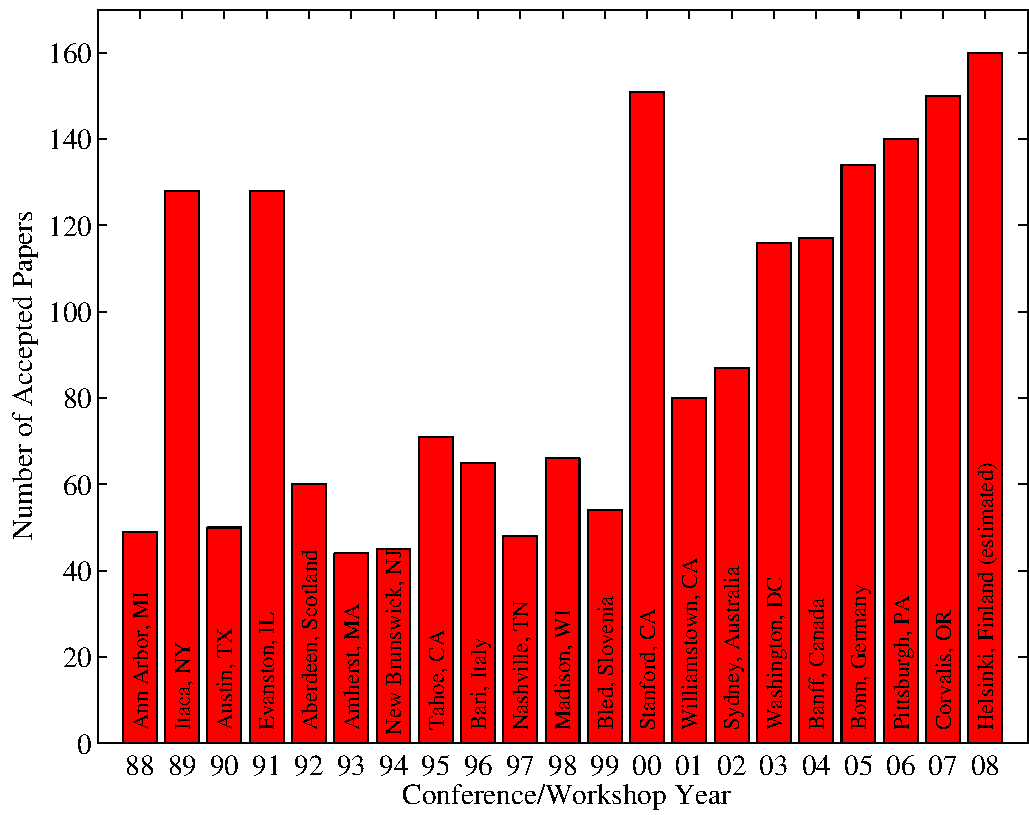
\includegraphics[width=\columnwidth]{icml_numpapers}}
%\caption{Historical locations and number of accepted papers for International
%Machine Learning Conferences (ICML 1993 -- ICML 2008) and International
%Workshops on Machine Learning (ML 1988 -- ML 1992). At the time this figure was
%produced, the number of accepted papers for ICML 2008 was unknown and instead
%estimated.}
%\label{icml-historical}
%\end{center}
%\vskip -0.2in
%\end{figure}

%\subsection{Figures}

%You may want to include figures in the paper to illustrate
%your approach and results. Such artwork should be centered,
%legible, and separated from the text. Lines should be dark and at
%least 0.5~points thick for purposes of reproduction, and text should
%not appear on a gray background.

%Label all distinct components of each figure. If the figure takes the
%form of a graph, then give a name for each axis and include a legend
%that briefly describes each curve. Do not include a title inside the
%figure; instead, the caption should serve this function.

%Number figures sequentially, placing the figure number and caption
%\emph{after} the graphics, with at least 0.1~inches of space before
%the caption and 0.1~inches after it, as in
%Figure~\ref{icml-historical}. The figure caption should be set in
%9~point type and centered unless it runs two or more lines, in which
%case it should be flush left. You may float figures to the top or
%bottom of a column, and you may set wide figures across both columns
%(use the environment \texttt{figure*} in \LaTeX). Always place
%two-column figures at the top or bottom of the page.

%\subsection{Algorithms}

%If you are using \LaTeX, please use the ``algorithm'' and ``algorithmic''
%environments to format pseudocode. These require
%the corresponding stylefiles, algorithm.sty and
%algorithmic.sty, which are supplied with this package.
%Algorithm~\ref{alg:example} shows an example.

%\begin{algorithm}[tb]
   %\caption{Bubble Sort}
   %\label{alg:example}
%\begin{algorithmic}
   %\STATE {\bfseries Input:} data $x_i$, size $m$
   %\REPEAT
   %\STATE Initialize $noChange = true$.
   %\FOR{$i=1$ {\bfseries to} $m-1$}
   %\IF{$x_i > x_{i+1}$}
   %\STATE Swap $x_i$ and $x_{i+1}$
   %\STATE $noChange = false$
   %\ENDIF
   %\ENDFOR
   %\UNTIL{$noChange$ is $true$}
%\end{algorithmic}
%\end{algorithm}

%\subsection{Tables}

%You may also want to include tables that summarize material. Like
%figures, these should be centered, legible, and numbered consecutively.
%However, place the title \emph{above} the table with at least
%0.1~inches of space before the title and the same after it, as in
%Table~\ref{sample-table}. The table title should be set in 9~point
%type and centered unless it runs two or more lines, in which case it
%should be flush left.

%% Note use of \abovespace and \belowspace to get reasonable spacing
%% above and below tabular lines.

%\begin{table}[t]
%\caption{Classification accuracies for naive Bayes and flexible
%Bayes on various data sets.}
%\label{sample-table}
%\vskip 0.15in
%\begin{center}
%\begin{small}
%\begin{sc}
%\begin{tabular}{lcccr}
%\toprule
%Data set & Naive & Flexible & Better? \\
%\midrule
%Breast    & 95.9$\pm$ 0.2& 96.7$\pm$ 0.2& $\surd$ \\
%Cleveland & 83.3$\pm$ 0.6& 80.0$\pm$ 0.6& $\times$\\
%Glass2    & 61.9$\pm$ 1.4& 83.8$\pm$ 0.7& $\surd$ \\
%Credit    & 74.8$\pm$ 0.5& 78.3$\pm$ 0.6&         \\
%Horse     & 73.3$\pm$ 0.9& 69.7$\pm$ 1.0& $\times$\\
%Meta      & 67.1$\pm$ 0.6& 76.5$\pm$ 0.5& $\surd$ \\
%Pima      & 75.1$\pm$ 0.6& 73.9$\pm$ 0.5&         \\
%Vehicle   & 44.9$\pm$ 0.6& 61.5$\pm$ 0.4& $\surd$ \\
%\bottomrule
%\end{tabular}
%\end{sc}
%\end{small}
%\end{center}
%\vskip -0.1in
%\end{table}

%Tables contain textual material, whereas figures contain graphical material.
%Specify the contents of each row and column in the table's topmost
%row. Again, you may float tables to a column's top or bottom, and set
%wide tables across both columns. Place two-column tables at the
%top or bottom of the page.

%\subsection{Citations and References}

%Please use APA reference format regardless of your formatter
%or word processor. If you rely on the \LaTeX\/ bibliographic
%facility, use \texttt{natbib.sty} and \texttt{icml2019.bst}
%included in the style-file package to obtain this format.

%Citations within the text should include the authors' last names and
%year. If the authors' names are included in the sentence, place only
%the year in parentheses, for example when referencing Arthur Samuel's
%pioneering work \yrcite{Samuel59}. Otherwise place the entire
%reference in parentheses with the authors and year separated by a
%comma \cite{Samuel59}. List multiple references separated by
%semicolons \cite{kearns89,Samuel59,mitchell80}. Use the `et~al.'
%construct only for citations with three or more authors or after
%listing all authors to a publication in an earlier reference \cite{MachineLearningI}.

%Authors should cite their own work in the third person
%in the initial version of their paper submitted for blind review.
%Please refer to Section~\ref{author info} for detailed instructions on how to
%cite your own papers.

%Use an unnumbered first-level section heading for the references, and use a
%hanging indent style, with the first line of the reference flush against the
%left margin and subsequent lines indented by 10 points. The references at the
%end of this document give examples for journal articles \cite{Samuel59},
%conference publications \cite{langley00}, book chapters \cite{Newell81}, books
%\cite{DudaHart2nd}, edited volumes \cite{MachineLearningI}, technical reports
%\cite{mitchell80}, and dissertations \cite{kearns89}.

%Alphabetize references by the surnames of the first authors, with
%single author entries preceding multiple author entries. Order
%references for the same authors by year of publication, with the
%earliest first. Make sure that each reference includes all relevant
%information (e.g., page numbers).

%Please put some effort into making references complete, presentable, and
%consistent. If using bibtex, please protect capital letters of names and
%abbreviations in titles, for example, use \{B\}ayesian or \{L\}ipschitz
%in your .bib file.

%\subsection{Software and Data}

%We strongly encourage the publication of software and data with the
%camera-ready version of the paper whenever appropriate. This can be
%done by including a URL in the camera-ready copy. However, do not
%include URLs that reveal your institution or identity in your
%submission for review. Instead, provide an anonymous URL or upload
%the material as ``Supplementary Material'' into the CMT reviewing
%system. Note that reviewers are not required to look at this material
%when writing their review.

%% Acknowledgements should only appear in the accepted version.
%\section*{Acknowledgements}

%\textbf{Do not} include acknowledgements in the initial version of
%the paper submitted for blind review.

%If a paper is accepted, the final camera-ready version can (and
%probably should) include acknowledgements. In this case, please
%place such acknowledgements in an unnumbered section at the
%end of the paper. Typically, this will include thanks to reviewers
%who gave useful comments, to colleagues who contributed to the ideas,
%and to funding agencies and corporate sponsors that provided financial
%support.


%% In the unusual situation where you want a paper to appear in the
%% references without citing it in the main text, use \nocite
%\nocite{langley00}

\bibliography{example_paper}
\bibliographystyle{icml2019}


%%%%%%%%%%%%%%%%%%%%%%%%%%%%%%%%%%%%%%%%%%%%%%%%%%%%%%%%%%%%%%%%%%%%%%%%%%%%%%%%
%%%%%%%%%%%%%%%%%%%%%%%%%%%%%%%%%%%%%%%%%%%%%%%%%%%%%%%%%%%%%%%%%%%%%%%%%%%%%%%%
%% DELETE THIS PART. DO NOT PLACE CONTENT AFTER THE REFERENCES!
%%%%%%%%%%%%%%%%%%%%%%%%%%%%%%%%%%%%%%%%%%%%%%%%%%%%%%%%%%%%%%%%%%%%%%%%%%%%%%%%
%%%%%%%%%%%%%%%%%%%%%%%%%%%%%%%%%%%%%%%%%%%%%%%%%%%%%%%%%%%%%%%%%%%%%%%%%%%%%%%%
%\appendix
%\section{Do \emph{not} have an appendix here}

%\textbf{\emph{Do not put content after the references.}}
%%
%Put anything that you might normally include after the references in a separate
%supplementary file.

%We recommend that you build supplementary material in a separate document.
%If you must create one PDF and cut it up, please be careful to use a tool that
%doesn't alter the margins, and that doesn't aggressively rewrite the PDF file.
%pdftk usually works fine. 

%\textbf{Please do not use Apple's preview to cut off supplementary material.} In
%previous years it has altered margins, and created headaches at the camera-ready
%stage. 
%%%%%%%%%%%%%%%%%%%%%%%%%%%%%%%%%%%%%%%%%%%%%%%%%%%%%%%%%%%%%%%%%%%%%%%%%%%%%%%%
%%%%%%%%%%%%%%%%%%%%%%%%%%%%%%%%%%%%%%%%%%%%%%%%%%%%%%%%%%%%%%%%%%%%%%%%%%%%%%%%


\end{document}


% This document was modified from the file originally made available by
% Pat Langley and Andrea Danyluk for ICML-2K. This version was created
% by Iain Murray in 2018, and modified by Alexandre Bouchard in
% 2019. Previous contributors include Dan Roy, Lise Getoor and Tobias
% Scheffer, which was slightly modified from the 2010 version by
% Thorsten Joachims & Johannes Fuernkranz, slightly modified from the
% 2009 version by Kiri Wagstaff and Sam Roweis's 2008 version, which is
% slightly modified from Prasad Tadepalli's 2007 version which is a
% lightly changed version of the previous year's version by Andrew
% Moore, which was in turn edited from those of Kristian Kersting and
% Codrina Lauth. Alex Smola contributed to the algorithmic style files.
